\documentclass[a4paper,11pt]{article}
\usepackage{iftex}
\ifPDFTeX\usepackage[utf8]{inputenc}\usepackage[T1]{fontenc}\else
\usepackage{fontspec}\usepackage{xeCJK}
\setCJKmainfont{HaranoAjiMincho-Regular.otf}\setCJKsansfont{HaranoAjiGothic-Medium.otf}
\fi
\usepackage{amsmath,amssymb,graphicx,booktabs,tabularx,array,float,hyperref,geometry,cite}
\geometry{margin=1in}
\hypersetup{hidelinks}
\emergencystretch=2em
\title{\vspace{0.5cm}\textbf{Spirit in Physics:}\\\large 反証可能な精神の物理仮説、パイロット実行可能性研究、\\および前向き検証framework}
\author{川崎 純$^{1}$・田井中一貴$^{2}$・竹内知倫$^{3}$\\
\small $^{1}$新潟大学大学院医歯学総合研究科\\
\small $^{2}$新潟大学脳研究所\\
\small $^{3}$オーフス大学 Department of Biomedicine\\
\small \texttt{root@junkawasaki.com}}
\date{2026年8月23日}

\begin{document}
\maketitle
\begin{abstract}
\emph{Spirit in Physics}は、精神が物理的に実現された情報担持組織であり、その構造を測定できるという作業仮説を提示する。参加者別応答多様体を操作的近似候補とし、応答エネルギー、ユング心理学的コンプレックス、集合的無意識に対応する共通成分を明示的な検証標的とする。Stage 1では反復言語連想測定から監査可能な幾何表現を構成できるかを検討した。参加者ディレクトリ11件のうち5名から、2セッション、共通刺激語99語、妥当な試行970件を得た。潜時の再検査相関は弱く（471組で$r=0.24$）、参加者間潜時相関は小さかった（$\bar r=0.065$、両側置換$p=0.038$）。第1主成分の分散比27\%は置換帰無分布の約26\%を上回らず（$p=0.21$）、ランク$[3,6,3]$テンソル近似は分散の75.9\%を記述した。そこで実行可能性結果にStage 2の前向き検証frameworkを組み合わせる。$H_{\mathrm{phys}}$を主要仮説、$H_{\mathrm{complex}}$と$H_{\mathrm{collective}}$を主要副次仮説、$H_{\mathrm{energy}}$を校正物理量を要する長期的機序仮説とする。独立追試、標本外予測、統制介入、外部構成概念妥当化、陰性対照、反証条件を事前規定する。Stage 1が支持するのは構成可能性であり、4仮説の証明ではない。
\end{abstract}

\section{はじめに}
言語連想課題における反応時間と自律神経反応は、刺激に伴う応答変動の研究に用いられてきた \cite{Jung1910}。グラフ法とテンソル法は、多変量観測を圧縮して記述する手段を与える \cite{KoldaBader2009}。ただし、数学的構成だけでは心理構成概念や因果機序は確立されない。

情報理論と情報処理の物理的コストは本研究の物理的前提を動機づける \cite{Shannon1948,Landauer1961,Berut2012}。長期的研究プログラムは、精神と呼ばれる情報組織が測定可能な物理的実現を持つかを問う。分析心理学とラバーハンド錯覚 \cite{Botvinick1998} は、その前提を検証するための候補構造と身体境界への介入を与える。

研究プログラムの目的は可視化に留まらず、精神の物理モデルを支持または反証し得る、再現可能で介入感受性のある証拠を蓄積することである。本稿の目的はその第1段階として、潜時と皮膚電位から監査可能な候補表現を構成できるか、また中心仮説のどこが未検証かを明確にすることである。

\section{作業前提と検証仮説}
本研究は、個人の精神が身体・認知状態からなる情報担持組織として物理的に実現される、という前提を採用する。測定多様体をただちに精神そのものと同一視するのではなく、予測、介入、追試によって妥当性を検証する候補モデルとする。Stage 2では$H_{\mathrm{phys}}$を主要仮説、$H_{\mathrm{complex}}$と$H_{\mathrm{collective}}$を主要副次仮説、校正物理量が得られるまで$H_{\mathrm{energy}}$を長期的機序仮説とする。

\begin{description}\small\setlength{\itemsep}{1pt}\setlength{\parsep}{0pt}
\item[$H_{\mathrm{phys}}$:] 精神が物理的実現を持つなら、推定状態は保留された行動・生理応答を再現可能に予測し、身体的自己や情報処理への統制介入に対して系統的に変化する。
\item[$H_{\mathrm{energy}}$:] より長い反応潜時と大きな自律神経変化を要する領域は、より高い応答コストの観測代理指標である。物理的エネルギーとして解釈するには、代理指標をエネルギーまたは情報熱力学量へ結ぶ校正測定が追加で必要である。
\item[$H_{\mathrm{complex}}$:] 安定した高コスト領域は、独立に評価した個人的に顕著なユング心理学的コンプレックスと対応し、領域構成に使っていない反応内容または生理を予測する。
\item[$H_{\mathrm{collective}}$:] 個人差と技術要因を制御した後も、追試可能な参加者間共通成分が残り、別標本へ一般化する。Jungの集合的無意識との対応は、理論が予測する意味・文化構造も示した場合にのみ支持される。
\end{description}

標本外予測、介入感受性、信頼性、独立した構成概念妥当性が得られなければ、対応する仮説への反証材料となる。本パイロットが主に検討するのは候補表現の構成可能性であり、その他の仮説に関する証拠は探索的である。

\section{Stage 1パイロット方法}
\subsection{倫理審査と同意}
プロジェクト資材には、新潟大学の承認（承認番号2024-0269、承認日2025年3月1日）が記載されている。研究画面は、研究目的、参加の任意性、不利益なく撤回できること、音声・映像記録への同意を登録前に求める。承認書原本と参加者別の同意記録は今回確認した解析packageに含まれていないため、投稿前に完全性を確認する必要がある。

\subsection{参加者と解析対象}
研究データには11名分のディレクトリが存在した。このうち、連続記録が取得不能なgit-annexポインタであった3名、連続生理CSVがなかった2名、課題イベントと記録時刻が重ならなかった1名を除外し、時刻整合した5名を解析した。これはデータ利用可能性に基づく部分集団であり、無作為または前向きに選ばれた標本ではない。人口学的・臨床的推論は行わない。

\subsection{課題と信号抽出}
参加者は約100語の刺激リストを2回実施した。本解析が用いるのは刺激語、イベント時刻、連続皮膚電位信号であり、発話された連想語の意味内容は多様体に使用していない。

Mod-002の連続CSV記録は1 Hzであった。反応潜時は\texttt{response\_window\_opened}から最初の\texttt{speech\_detected}までとし、$0<\mathrm{latency}<12$秒を満たすものを採用した。各チャンネルの皮膚電位変化$\Delta SP$は、刺激表示前3秒の平均を基準とする応答窓内の最大絶対偏差とした。イベント時刻が記録内にあり、4チャンネルすべての窓が利用可能な試行のみを残した。妥当な試行は計970件で、参加者別には198、181、195、199、197件であった。

現行解析コードではCh2を主皮膚電位チャンネルとし、Ch1もテンソル特徴として保持する。この選択は事前登録されておらず、各チャンネルに安定した生理学的意味を与える電極配置メタデータも解析資材には十分含まれていなかった。

\subsection{参加者別応答空間}
参加者内で試行を刺激語ごとに平均し、反応潜時、$\Delta SP_{Ch1}$、$\Delta SP_{Ch2}$の3特徴を用いた。可視化のため、記述的な応答コスト得点を
\begin{equation}
C(w)=z\{\mathrm{latency}(w)\}+z\{\Delta SP_{Ch2}(w)\}
\end{equation}
と定義した。これは$H_{\mathrm{energy}}$における無次元の候補代理指標であり、物理的エネルギーの直接測定ではない。妥当化には独立したエネルギーまたは情報熱力学測定が必要である。

特徴標準化後、二乗ユークリッド距離から
\begin{equation}
W_{ij}=\exp\{-\lVert x_i-x_j\rVert^2/\sigma^2\}
\end{equation}
を作り、$\sigma$は非ゼロの単語間距離の中央値とした。対称正規化グラフLaplacian $L_{sym}=I-D^{-1/2}WD^{-1/2}$ の低次非自明固有ベクトルを座標とした。これはグラフ・スペクトル応答埋め込みであり、Fisher計量に基づく情報幾何学ではない。

\subsection{コホートテンソルと探索的統計}
参加者別・単語別平均を$\mathcal{T}\in\mathbb{R}^{P\times W\times F}$（$P=5,W=99,F=3$）にした。欠測セルはまず単語--特徴平均、次に特徴平均で補完し、特徴ごとに参加者--単語平面全体で標準化した。切断HOSVD/Tucker近似 \cite{KoldaBader2009} のランクは$[3,6,3]$とした。グラフスペクトル、participation ratio、再構成分散は、独立標本でランク選択されていない記述量である。

再検査安定性は、対応するセッション1・2の潜時のPearson相関とした。参加者間構造は参加者$\times$単語の潜時行列で評価した。平均非対角Pearson相関と第1主成分分散比を、seed 7、2,000回の参加者内単語置換による帰無分布と比較した。相関検定は両側である。解析は探索的かつ事前登録されておらず、多重性調整済みの確証的主張は行わない。

\section{Stage 2前向き検証framework}
次の大規模dataset研究を前向き検証段階として計画する。本節はframeworkであって、完了した事前登録ではない。確証データを確認する前に、protocol、code version、endpoint定義、効果方向、成功閾値、除外、欠測処理、解析順序を公開registryにtimestamp付きで固定する。

\subsection{研究design、cohort、sample size}
Stage 2では、信頼性と標本外予測を推定できる反復測定を行う。Stage 1の不安定な効果量を真値として扱わず、想定する信頼性、脱落、cluster、効果量の範囲を用いたsimulationでsample sizeを決める。discovery cohortと独立replication cohortを分離し、文化的一般化を主張する場合は別言語または別文化cohortを追加する。割付、介入順序、device version、sensor配置、校正、取得失敗を機械可読のparticipant flowに保存する。

\subsection{前向き判定表}
\begin{table}[H]
\centering\footnotesize
\caption{\textbf{前向き検証logic。} 正確なendpointと閾値は確証データ確認前に固定する。}
\begin{tabularx}{\textwidth}{>{\raggedright\arraybackslash}p{0.12\textwidth} >{\raggedright\arraybackslash}X >{\raggedright\arraybackslash}X >{\raggedright\arraybackslash}X}
\toprule
仮説 & 主要validation & 必須比較 & 仮説への反証材料 \\
\midrule
$H_{\mathrm{phys}}$ & 標本外の行動・生理予測と事前規定した身体的自己への介入 & 個人非依存、語彙、sham、無介入baseline & 追加予測力または再現可能な介入変化がない \\
$H_{\mathrm{energy}}$ & $C$と独立に校正したエネルギーまたは情報熱力学量との関連 & 潜時のみ、覚醒のみ、非エネルギー交絡model & 交絡制御後に独立物理量との関連がない \\
$H_{\mathrm{complex}}$ & 高$C$領域が盲検・独立測定した個人的salienceまたはcomplex基準を予測 & 単語頻度、感情価、潜時、皮膚電位成分 & 信頼性または外部追加予測力がない \\
$H_{\mathrm{collective}}$ & 事前規定した共有意味構造が独立・異文化標本で再現 & shuffle、語彙頻度、言語、device、site、人口学的baseline & 制御後に成分が消える、または外部追試に失敗 \\
\bottomrule
\end{tabularx}
\label{tab:stage2}
\end{table}

\subsection{解析階層とdata leakage防止}
信頼性を最初のgateとし、不安定な表現を強い構成概念主張へ進めない。主要$H_{\mathrm{phys}}$解析では参加者単位でtrain、validation、testを分離し、前処理はtrain partition内で推定する。baselineと陰性対照を同一の保留観測で比較する。必要に応じてparticipant、word、session、site、deviceを階層modelで扱う。主要解析後に主要副次仮説を検定し、多重性制御、方向contrast、Bayesian判定基準を登録時に固定する。探索的解析は明示し、成功定義を変更しない。

\subsection{証拠level}
累積的証拠を、Level 0：構成可能性（本pilot）、Level 1：再検査信頼性、Level 2：標本外予測、Level 3：統制介入への応答、Level 4：独立したエネルギー・complex妥当性、Level 5：共有構造の独立・異文化追試、と定義する。精神の物理modelを支持するには少なくともLevel 3、集合的無意識の解釈にはLevel 5と事前規定した意味・文化構造を要求し、主成分分散比だけでは判定しない。

\subsection{事前登録と公開}
登録または確証データへのaccess前に、Stage 2を固定解析commitとともに事前登録する。公開packageにはversion固定環境、checksum、syntheticまたは倫理上公開可能な派生test data、participant flow、endpoint辞書、単一commandの再現経路を含める。匿名化派生結果とcodeには永続archive identifierを付与し、参加者mediaは同意と倫理承認に従って管理する。

\section{Stage 1パイロット結果}
\subsection{試行レベルの応答分布}
改訂図1には妥当な970試行すべてを示し、パーセンタイルによる表示除外は行っていない。色は図の2軸から計算されるため、低い$C$と高い$C$の分離は定義上期待される。これは測定範囲を示すが、潜在クラスの証拠ではない。潜時の再検査相関は弱かった（$r=0.24$、対応する参加者--単語471組）。

\begin{figure}[t]
\centering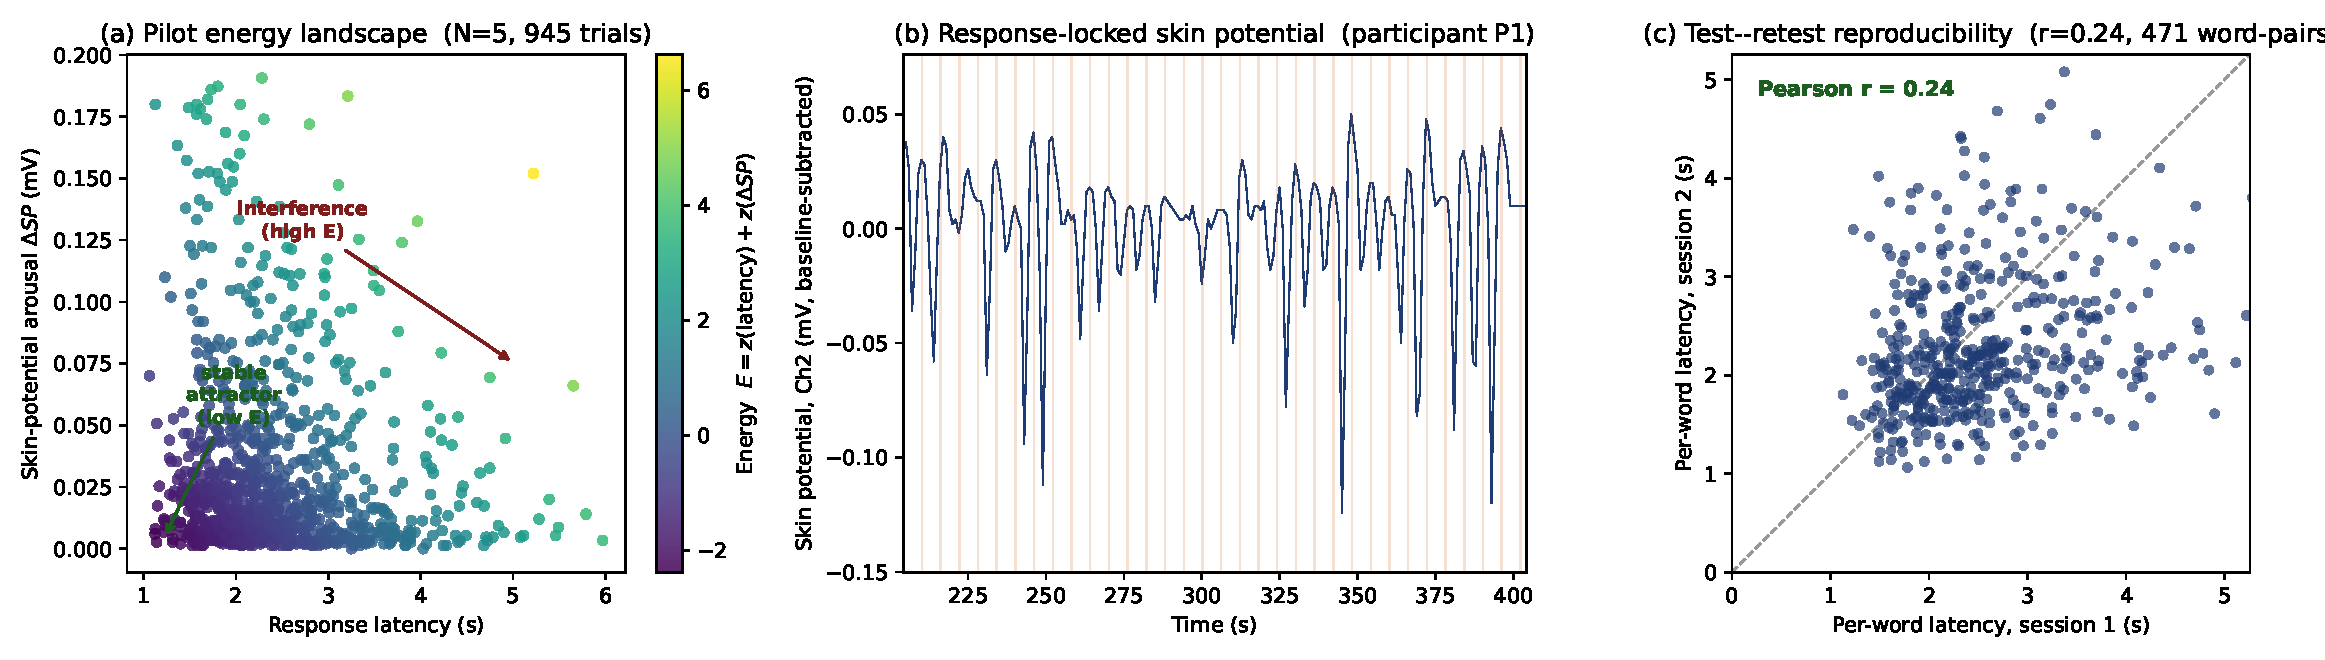
\includegraphics[width=\textwidth]{fig_landscape.pdf}
\caption{\textbf{パイロット測定。} (a) 妥当な970試行の反応潜時とCh2皮膚電位変化。色は記述的応答コスト得点$C$。(b) 連続皮膚電位の例と課題イベント。(c) 対応する参加者--単語におけるセッション1・2の潜時。}
\label{fig:landscape}
\end{figure}

\subsection{参加者別埋め込み}
同一アルゴリズムで参加者ごとの2次元応答埋め込みを得た（図\ref{fig:individual}）。$H_{\mathrm{complex}}$の下では、安定した高$C$領域がコンプレックスの候補指標となる。ただしパネル間の視覚差は記述的であり、本パイロットには独立したコンプレックス評価または検証済み分類器がない。

\begin{figure}[t]
\centering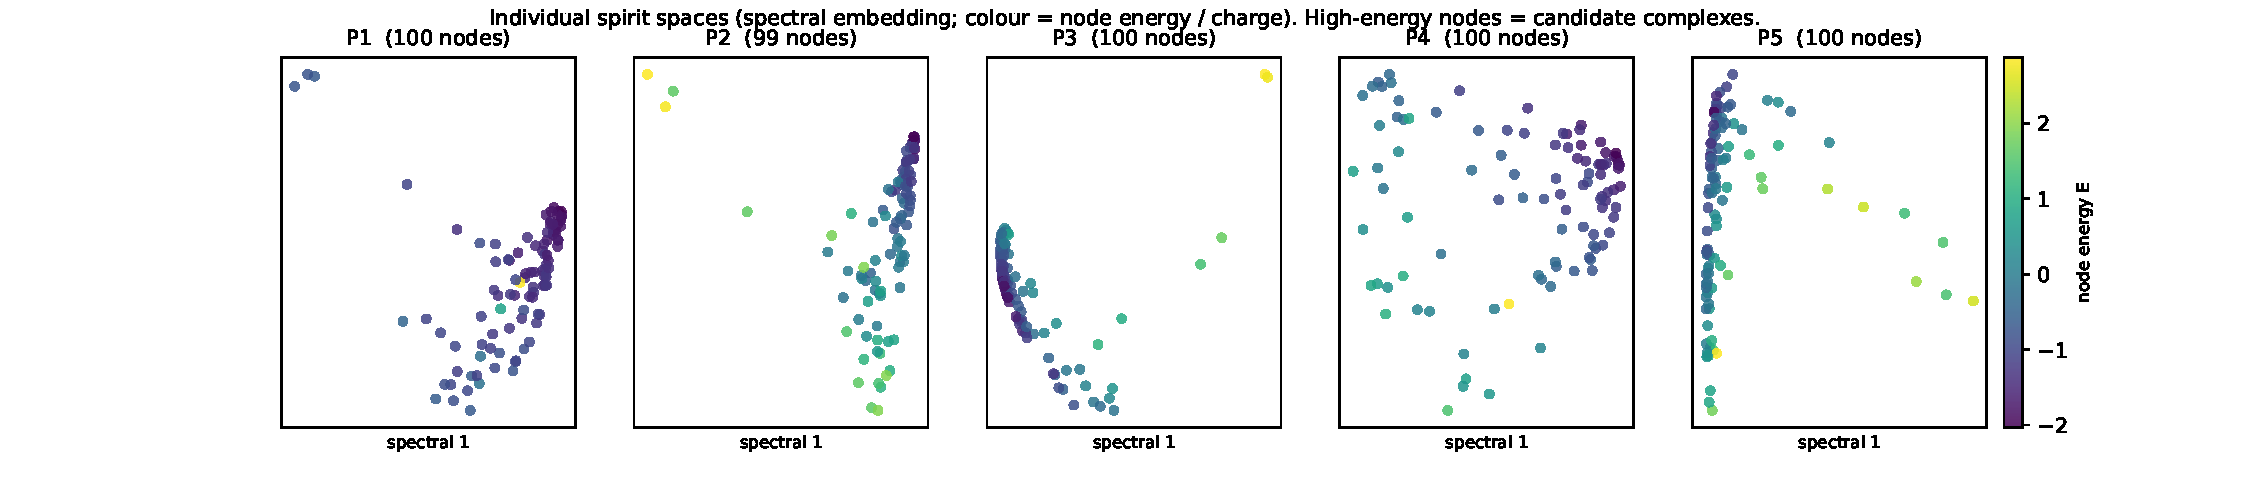
\includegraphics[width=\textwidth]{fig_individual_spirit.pdf}
\caption{\textbf{参加者別応答空間。} 各パネルは潜時と2つの皮膚電位特徴による単語ノードのグラフ・スペクトル埋め込み。色は$C$。軸の符号と向きは任意で、整列なしに直接比較できない。}
\label{fig:individual}
\end{figure}

\subsection{参加者間潜時とテンソルの要約}
参加者間潜時相関の平均は$\bar r=0.065$で、両側置換検定は$p=0.038$であった。第1主成分は27\%を説明したが、置換帰無平均の約26\%と近く、$p=0.21$であった（図\ref{fig:collective}）。これは$H_{\mathrm{collective}}$に関係する微弱な探索的観測であるが、主成分結果は大きな共通成分を支持せず、仮説が要求する意味構造も未検証である。

\begin{figure}[t]
\centering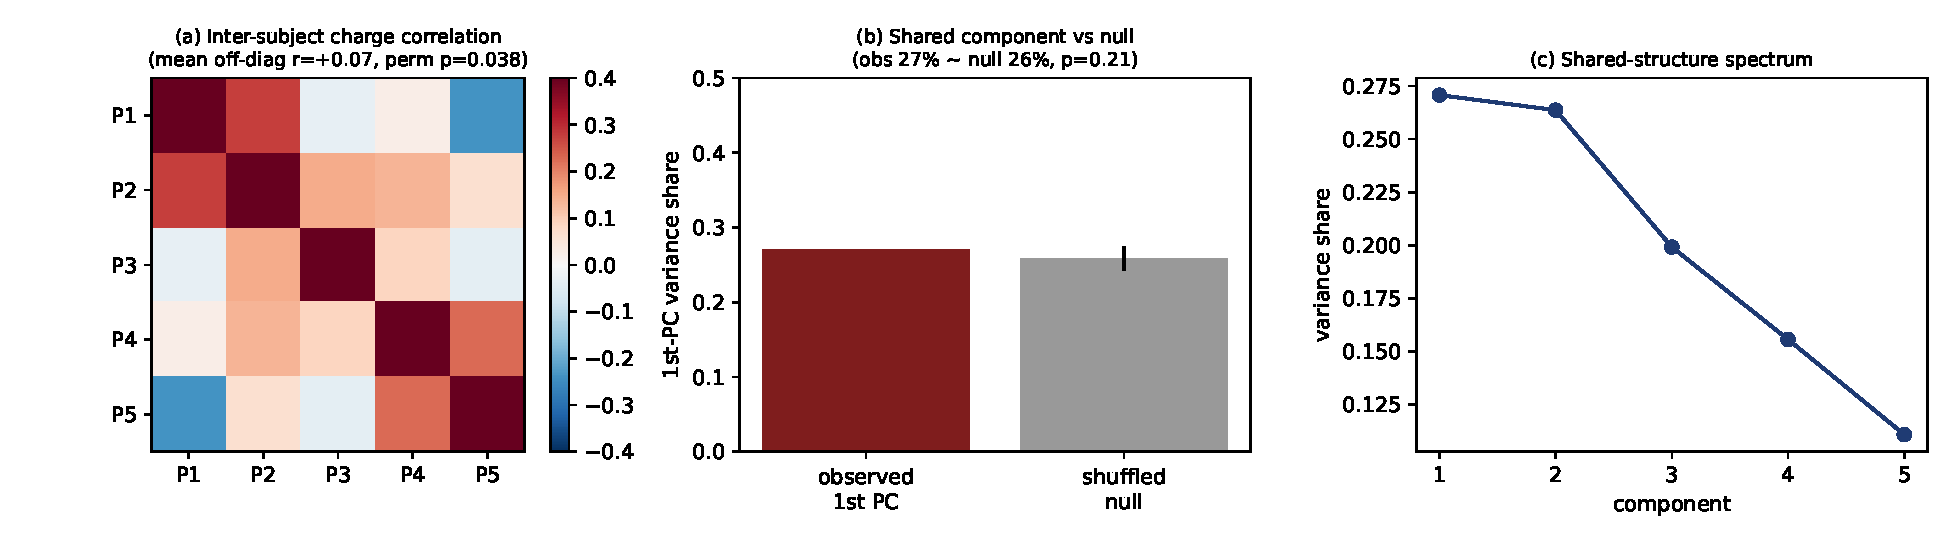
\includegraphics[width=\textwidth]{fig_collective.pdf}
\caption{\textbf{探索的な参加者間潜時解析。} (a) ペア相関と平均および参加者内両側置換検定。(b) 第1主成分分散比と置換帰無分布。(c) 潜時の分散スペクトル。解析対象は潜時であり、生理的「charge」ではない。}
\label{fig:collective}
\end{figure}

テンソル形状は$5\times99\times3$、中央値距離カーネルの$\sigma=4.2109$、グラフ固有値ギャップ0.1948、participation ratio 10.89であった。ランク$[3,6,3]$ HOSVDは分散の75.9\%を再構成した（図\ref{fig:manifold}）。参加者5名、特徴3個という制約がこれらの値に影響するため、集団多様体や一意な「集合座標」を確立しない。

\begin{figure}[t]
\centering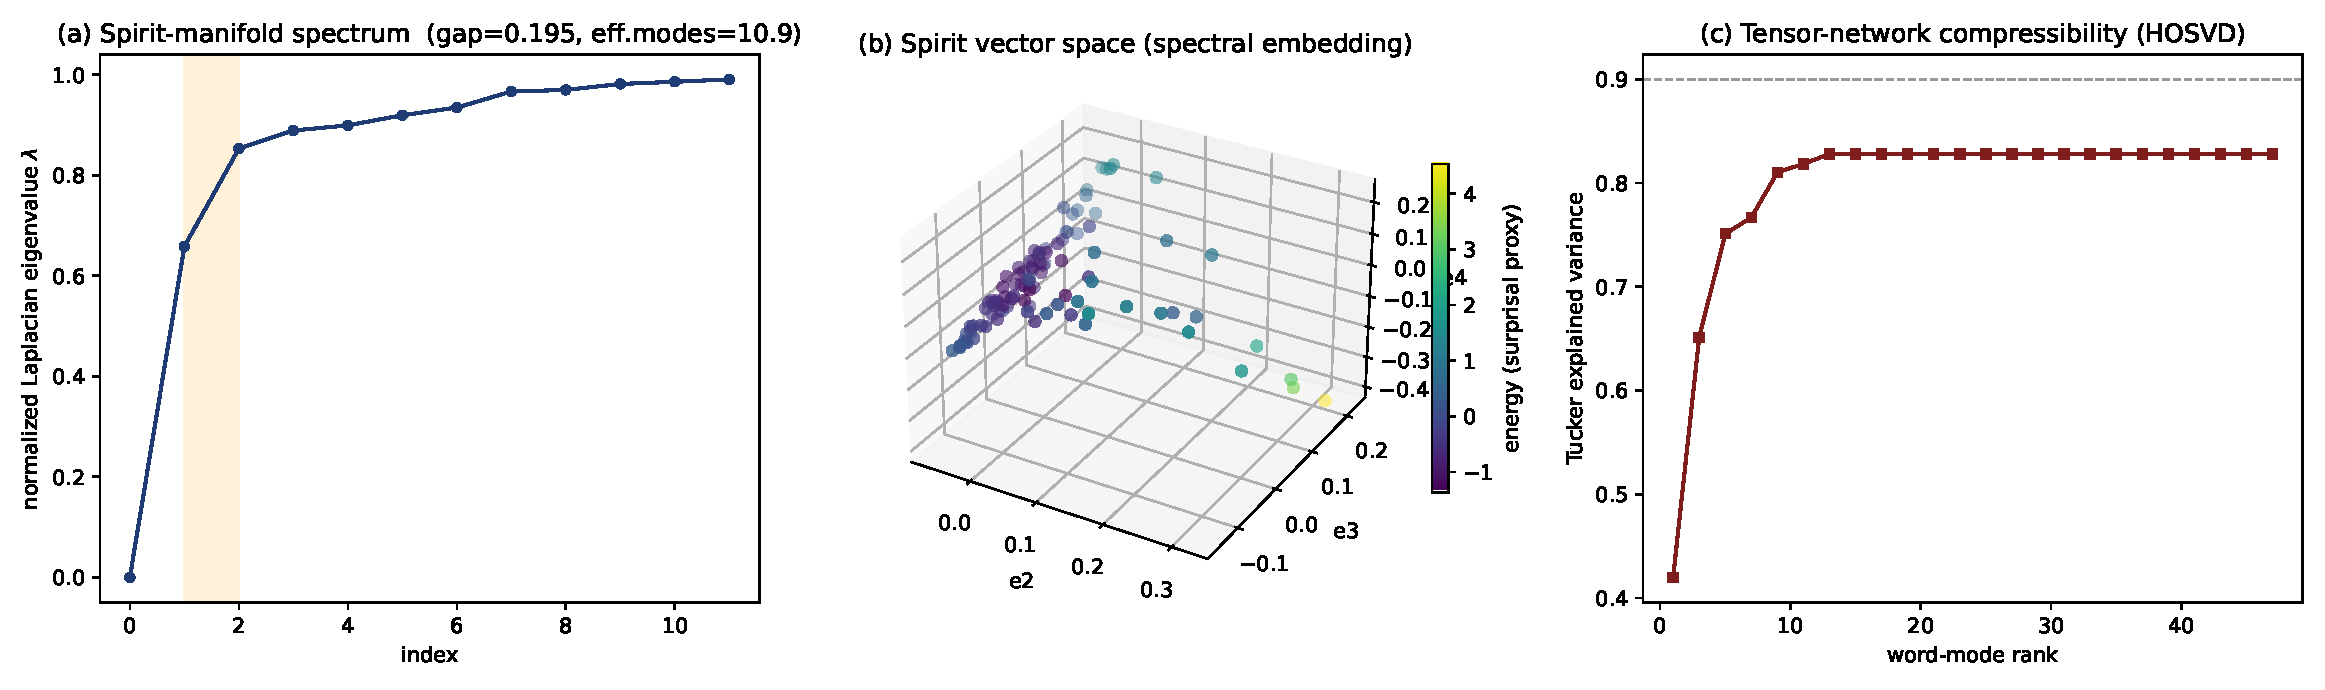
\includegraphics[width=\textwidth]{fig_spirit_manifold.pdf}
\caption{\textbf{記述的コホート幾何。} $5\times99\times3$テンソルのグラフLaplacianスペクトル、3次元単語埋め込み、Tucker再構成曲線。すべて標本内の記述量である。}
\label{fig:manifold}
\end{figure}

\section{考察}
4仮説は解析後の装飾的解釈ではなく、本研究プログラムの科学的中心である。Stage 1は、時刻整合した言語連想課題と皮膚電位データを、監査可能な計算により参加者別グラフ埋め込みとコホートテンソルへ変換できることを示した。Stage 2は、研究を信頼性、予測、介入、独立妥当化、追試の前向き系列へ変換するもので、結論をあらかじめ決めるものではない。

物理的前提は、識別力のある測定によって初めて科学的になる。本稿では温度、熱、仕事、消去事象、エントロピー生成を測っていないため、$C$はエネルギー仮説の代理指標であって熱力学的エネルギーではない。またRBFグラフは最初の操作的幾何であり、Fisher計量の統計多様体ではない。$H_{\mathrm{phys}}$と$H_{\mathrm{energy}}$を支持するには、今後の研究で候補空間を校正されたエネルギー量と統制介入へ結ぶ必要がある。

弱い再検査相関は、測定誤差、学習、状態変化、時刻整合の影響が大きい可能性を示す。小さな置換結果は、小規模な完全記録部分集団をデータ確認後に解析し、多重性を制御しておらず、PC解析も帰無であったため、仮説生成に留める。次の研究では主チャンネルと得点を事前規定し、電極配置・校正情報と参加者フローを保存し、除外基準を解析前に定め、信頼性を推定し、保留セッションまたは外部転帰で検証すべきである。

\section{限界}
解析標本は11名中5名で、ローカルデータの利用可能性に依存した。取得不能なannexオブジェクト、記録欠如、時刻不整合は選択バイアスを生じ得る。1 Hzサンプリングは時間的解釈を制限する。チャンネル選択は事前登録されず、センサーメタデータは不完全で、陰性対照刺激や独立検証cohortはなかった。連想応答の意味内容とラバーハンド錯覚データは解析していない。統計は探索的で、複数の解析選択に対する調整はない。Stage 2 framework自体は事前登録ではなく、endpoint、閾値、sample size、介入、data governanceは研究者と倫理審査の承認後に固定する必要がある。現リポジトリは公開されておらず、匿名化派生データも永続的公開archiveに未登録である。

\section{データとコードの利用可能性}
解析コード、イベント処理ロジック、原稿ソースはプロジェクトリポジトリで管理している。本preprint時点でリポジトリは非公開で、参加者レベル記録も公開していない。独立再現可能と記載する前に、匿名化派生表、version固定コード、環境仕様、checksumを永続的アーカイブへ登録する必要がある。元研究データへのアクセスは倫理承認、同意、適切なデータ利用手続に従い、問い合わせは責任著者が受け付ける。

\section{結論}
本preprintは、精神の物理仮説に関するStage 1実行可能性結果とStage 2前向き検証frameworkを統合した。物理的実現、応答エネルギー、ユング心理学的コンプレックス、集合的無意識をgate付き累積証拠programの明示的標的とする。現在のデータはLevel 0の構成可能性を確立し、事前登録した信頼性、標本外予測、統制介入、エネルギー校正、独立構成概念妥当性、追試によって仮説を進めるかを判定する。

\section*{著者の貢献}
J.K.は研究を着想し、パイロットデータ収集、解析実装、原稿執筆を行った。K.T.とT.T.は科学的指導と批判的解釈に貢献した。投稿前に全著者が最終原稿を確認し承認する必要がある。

\section*{研究費と利益相反}
研究費と利益相反は投稿前に全著者が確認する必要がある。本稿では未確認の宣言を記載しない。

\begingroup\footnotesize
\bibliographystyle{unsrt}
\bibliography{references}
\endgroup
\end{document}
